%----------------------------------------------------------------------------------------------------=
%-----------------------------------------------------------------------------------------------------
% Define Document Class, and include/import the multiple libraries used to create this document 
%-----------------------------------------------------------------------------------------------------
\documentclass[12pt]{article}
\usepackage{amsmath}
\usepackage[sc]{mathpazo}
\usepackage{geometry}
\usepackage{datetime}
\usepackage[myheadings]{fullpage}
\usepackage{fancyhdr}
\usepackage{lastpage}
\usepackage{graphicx, wrapfig, subcaption, setspace, booktabs}
\usepackage[T1]{fontenc}
\usepackage[font=small, labelfont=bf]{caption}
\usepackage{fourier}
\usepackage[protrusion=true, expansion=true]{microtype}
\usepackage[english]{babel}
\usepackage{sectsty}
\usepackage{url, lipsum}
\usepackage{hyperref,bookmark}
\usepackage[T1]{fontenc}
\usepackage{amssymb}
\usepackage{listings}
\usepackage{xcolor}
\usepackage{tabularx}
\usepackage{longtable}
\usepackage{setspace}
\usepackage{float}
\usepackage{bigfoot} % to allow verbatim in footnote
\usepackage[framed,numbered,autolinebreaks,useliterate]{matlab-prettifier}
\usepackage{filecontents}
\usepackage[ruled,linesnumbered]{algorithm2e}

%-----------------------------------------------------------------------------------------------------
% Define the heading for this document
%-----------------------------------------------------------------------------------------------------
% Heading style, calling fancy header library
\pagestyle{fancy}
\fancyhf{}
\setlength\headheight{15pt}
%%%% PUT YOUR NAME HERE FOR YOUR HEADING %%%%
\fancyhead[L]{Luis Fernando Enriquez-Contreras}
\fancyhead[R]{EE 105 Lab 3 Solution}
\fancyfoot[R]{Page \thepage\ of \pageref{LastPage}}

%-----------------------------------------------------------------------------------------------------
% Set coding for in LaTeX for Matlab
%-----------------------------------------------------------------------------------------------------
\lstset{
	style              = Matlab-editor,
	basicstyle         = \mlttfamily,
	escapechar         = ",
	mlshowsectionrules = true
}

% The workflow of the document begins here
\begin{document}
	%-------------------------------------------------------------------------------
	% Title
	%-------------------------------------------------------------------------------
	\begin{titlepage}
		
		\newcommand{\HRule}{\rule{\linewidth}{0.5mm}} % Defines a new command for the horizontal lines, change thickness here
		
		\center % Center everything on the page
		
		%---------------------------------------------------------
		%	HEADING SECTIONS
		%---------------------------------------------------------
		
		\textsc{\LARGE University of California, Riverside}\\[1.5cm] % Name of your university/college
		\textsc{\Large Bourns College of Engineering}\\[0.5cm] % Major heading such as course name
		\textsc{\large Department of Electrical and Computer Engineering}\\[0.5cm] % Minor heading such as course title
		
		%---------------------------------------------------------
		%	TITLE SECTION
		%---------------------------------------------------------
		
		\HRule \\[0.6cm]
		{\Large EE 105 Lab 3 Solution \\ \normalsize First-order systems in Simulink}\\[0.4cm] % Title of your document
		\HRule \\[1.0cm]
		
		%---------------------------------------------------------
		%	AUTHOR SECTION
		%---------------------------------------------------------
		
		%\begin{minipage}{0.4\textwidth}
		\begin{center} \large
			% \emph{Authors:}  
			\medskip
			%%% PUT YOUR NAME HERE %%%
			{\textsc{\textbf{Luis Fernando Enriquez-Contreras} }} 
		\end{center}
		%\end{minipage}
		
		
		%---------------------------------------------------------
		%	DATE SECTION
		%---------------------------------------------------------
		\begin{center}
			%			\selectlanguage{USenglish}
			{\large }
		\end{center}
		% Date, change the \today to a set date if you want to be precise
		
		%---------------------------------------------------------
		%	LOGO SECTION
		%---------------------------------------------------------
		%\vfill
		\newcommand*{\plogo}{
\includegraphics{Code/Fig/UC_Riverside_seal.pdf}}
		%		\newcommand*{\plogo}{
\includegraphics[width=0.25\textwidth]{UC_Riverside_seal.pdf}}
		
		\plogo\\[1cm] % Include a department/university logo - this will require the graphicx package
		
		%---------------------------------------------------------
		
		\vfill % Fill the rest of the page with whitespace
	\end{titlepage}
	
	\newpage
	
	%-------------------------------------------------------------------------------
	% Table of Contents and Figures
	%-------------------------------------------------------------------------------
	%	\doublespacing
	\tableofcontents
	\pagebreak
	\listoffigures
	%	\listoftables
	\lstlistoflistings  
	\pagebreak
	
	%-------------------------------------------------------------------------------
	% BODY
	%-------------------------------------------------------------------------------
	
	\section{Introduction}
	%%% PUT INTRODUCTION HERE %%%
	This laboratory introduces Simulink through the analysis and design of linear ordinary differential equations (ODEs). You will explore key systems concepts like transfer functions, time constants, pole locations, DC gain, and frequency response. The design process involves choosing system parameters to meet specific requirements, using transfer functions for analysis and state-space representation for simulation testing. The lab starts with fundamental concepts in first-order systems and progressively generalizes them to higher-order systems.
	
	
	\section{Pre-Lab}
		%%% Insert Figure Here as a .pdf File %%%
		\subsection{Part 1}
			\begin{figure}[H]
			\centering
			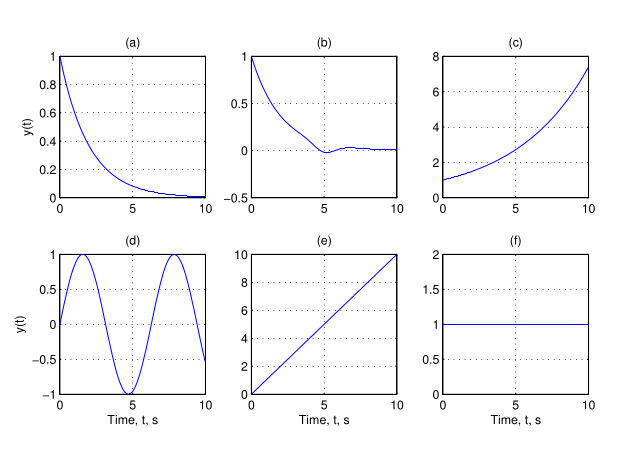
\includegraphics[width=1\linewidth]{"Code/Fig/prelab_part1.png"}
			\caption{Figures for the Prelab Part 1}
			\label{fig:prelab}
		\end{figure}
		\begin{itemize}
			\item Only graphs (a), (c), and (f) from Figure \ref{fig:prelab} could correspond to a first order linear system, as none of the other graphs were exponential.
			\begin{itemize}
				\item (f) Parameter $a$ has the value zero, and thus never decays.
				\item (c)  has a positive value for its parameter a, thus the system is unstable
				\item (a)  has a negative value for a, thus it is stable. We can then use the initial value of that graph,
				y(0) = 1, $a$ = -.460517 therefore, $\tau$ = 2.2 seconds
			\end{itemize}
			\item (b) Graphs (b), (d), and (e) did not match the form of a decaying function.
		\end{itemize}
		
		\subsection{Part 2}
		The transfer function for the circuit is seen in Equation \ref{eq:tf}.
		\begin{equation} \label{eq:tf}
			\begin{aligned}
				\mathrm{H}(\mathrm{s})=\mathrm{Y}(\mathrm{s}) / \mathrm{U}(\mathrm{s})=\frac{1}{s R C+1} \\ 	\mathrm{H}(\mathrm{s})=\mathrm{Y}(\mathrm{s}) / \mathrm{U}(\mathrm{s})=\frac{\frac{1}{R C}}{s+\frac{1}{R C}}
			\end{aligned}
		\end{equation}
		\begin{equation} \label{eq:ssgen}
			\begin{aligned}
				\dot{x} & = [a] x + [b] u \\
				y & =[c] x + [d] u
			\end{aligned}
		\end{equation}
		\begin{equation} \label{eq:ss}
			\begin{aligned}
				\dot{x} & =\left[\frac{-1}{\mathrm{RC}}\right] x+\left[\frac{1}{\mathrm{RC}}\right] u \\
				y & =[1] x + [0] u
			\end{aligned}
		\end{equation}
		The state space for the RC circuit is shown in Equation \ref{eq:ss}. Knowing the layout of a state pace model as shown in Equation \ref{eq:ssgen}, a = -10, b = 10, and c =  1.
		\subsection{Part 3}
		\begin{equation} \label{eq:mag_ang}
			M(w) = |H(j \omega)| = \frac{c b}{\sqrt{a^2+\omega^2}} \quad \text { and } \quad \Phi(\omega) = \angle H(j \omega) = \tan ^{-1}\left(\frac{\omega}{a}\right)
		\end{equation}
		Using equation \ref{eq:mag_ang} from the lab manual, the Magnitude and Phase for this RC Circuit is calculated in Equation : 
		\begin{equation} \label{eq:}
			\begin{aligned}
				\quad|H(j \omega)| & = \frac{10}{\sqrt{100+\omega^2}} \\
				\quad \angle H(j \omega) & = \arctan (-\omega / 10) \\
			\end{aligned}
		\end{equation}
		Plugging in $\omega$ = 10 and $a$  = -10, $\quad|H(j \omega)|$ = $\frac{100}{\sqrt{200}}$ = 0.707, and $ \tan ^{-1}\left(\frac{10}{-10}\right)$ = $-45^{\circ}$. The other $\omega$s are calculated in Table \ref*{tab:rc}.
		\begin{table}[H]
			\centering
			\caption{Magnitude and Phase for RC Circuit}
		\begin{tabular}{|c|c|c|c|c|}			
			\hline$\omega, \mathrm{rad} / \mathrm{s}$ & $|H(j \omega)|$ & $20 \log |H(j \omega)|$ & $\angle H(j \omega) \mathrm{rad}$ & $\angle H(j \omega)$ deg \\
			\hline 0.00 & 1 & 0 $ d B$ &  0.00 & $0^{\circ}$ \\
			\hline 0.01 & 1& 0 $ d B$ & -0.001 & $-0.057^{\circ}$ \\
			\hline 0.10 & 1  & 0 $ d B$ & -0.01 & $-0.573^{\circ}$ \\
			\hline 1.00 &  0.995  &-0.043 $ d B$ & -0.1 & $-5.711^{\circ}$ \\
			\hline 10.00 &  0.707 & -3.01 $ d B$ & -0.785 & $-45^{\circ}$ \\
			\hline 100.00 & 0.1 & -20.43 $ d B$ & -1.471  & $-84.289^{\circ}$ \\
			\hline
		\end{tabular}
		\label{tab:rc}
	\end{table}
		\subsection{Part 4}
		\begin{figure}[H]
			\centering
			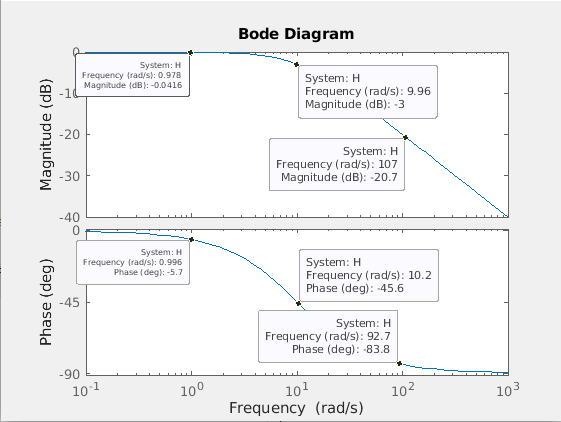
\includegraphics[width=1\linewidth]{"Code/Fig/prelab_bode_label.png"}
			\caption{Bode Plot for RC Circuit}
			\label{fig:bode}
		\end{figure}
		Figure \ref{fig:bode} matches the values in Table \ref{tab:rc}. 
		\newpage
	\section{Time Constant Estimation}
		%%% INSERT CODE HERE AS A .m FILE %%%
		\lstinputlisting[language=Matlab, caption = {\Large Matlab Code for Time Constant Estimation}]{"Code/time_constant_estimation.m"}	
			$\tau$  from both methods in the code is $\approx$ 0.15.
		%%% Insert Figure Here as a .pdf File %%%
		\begin{figure}[H]
			\centering
			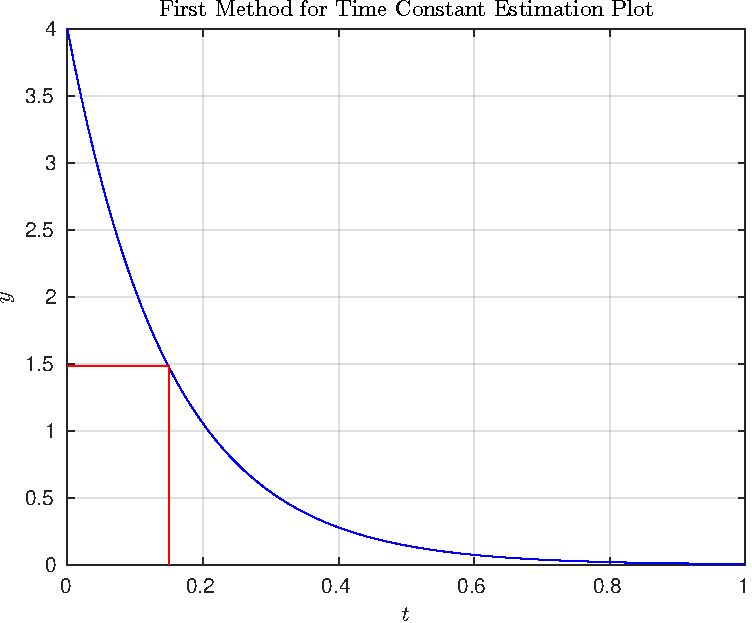
\includegraphics[width=1\linewidth]{"Code/Fig/first_method_time_constant_plot_line.pdf"}
			\caption{First Method Time Constant Estimation Plot}
			\label{fig:first_method_time_constant_plot}
		\end{figure}
		% Answer questions pertaining to the section below
	  	Figure \ref{fig:first_method_time_constant_plot} finds $\tau$ by looking for 37\% of the original value. Using 0.37 $\times$ 4 is $\approx$ 1.48 to find the y value, x occurs 0.15 s.
	  	\begin{figure}[H]
	  		\centering
	  		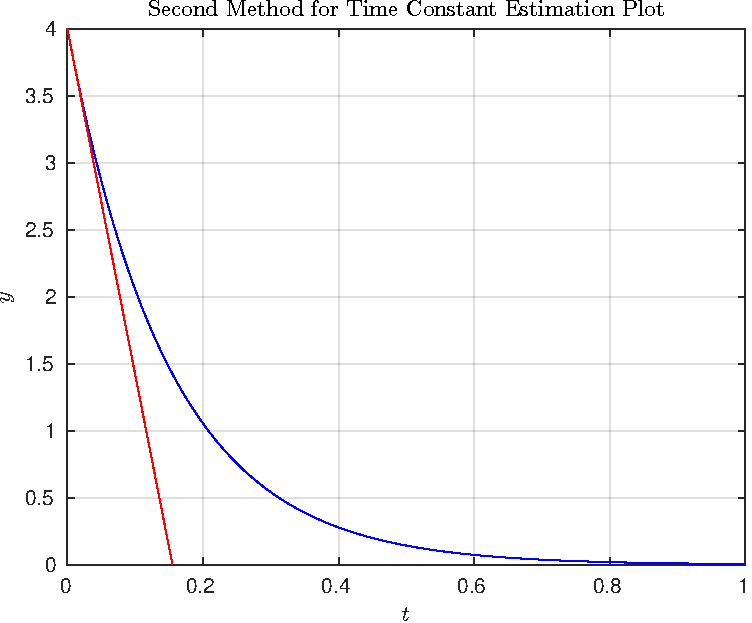
\includegraphics[width=1\linewidth]{"Code/Fig/second_method_time_constant_plot_line.pdf"}
	  		\caption{Second Method Time Constant Estimation Plot}
	  		\label{fig:second_method_time_constant_plot}
	  	\end{figure}
  		Figure \ref{fig:second_method_time_constant_plot} calculates $\tau$ by finding the slope of the curve at $t$ = 0. The slops crosses the x-axis at $\approx$ 0.15, so both methods concur that $\tau$ should be $\approx$ 0.15.
	\section{Simulation with Simulink}
		\subsection{Zero Input Response}
			\begin{figure}[H]
				\centering
				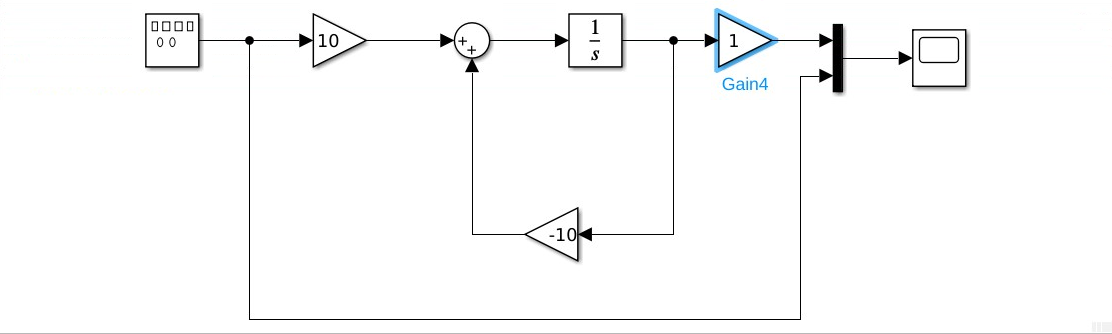
\includegraphics[width=1\linewidth]{"Code/Fig/part2_1_slx.png"} % Does not have to be a .pdf, can be another image file
				\caption{Simulink Diagram for Zero Input Response}
				\label{fig:slx_zero_input_diagram}
			\end{figure}	
			%%% Insert Figure Here as a image File %%%
			\begin{figure}[H]
				\centering
				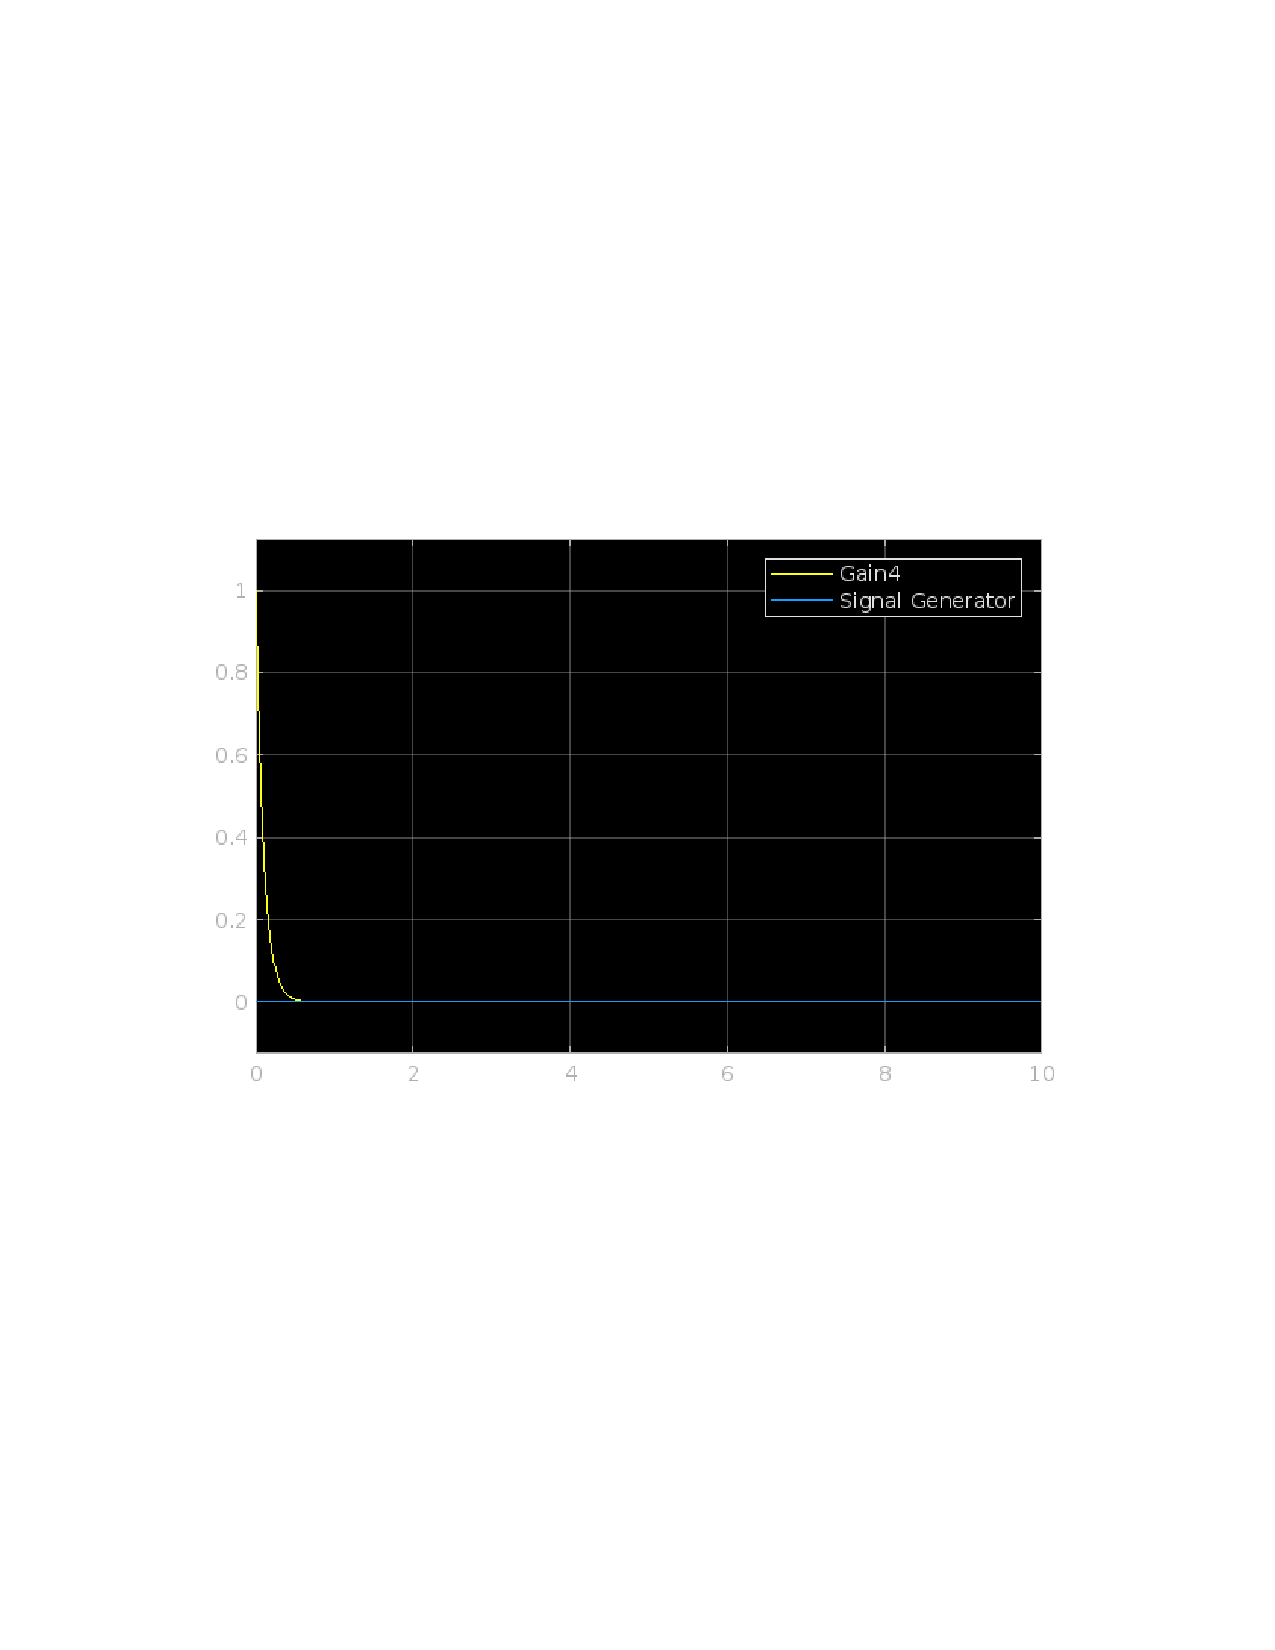
\includegraphics[width=0.8\linewidth]{"Code/Fig/zero_input_output.png"} 
				\caption{Oscilloscope Output of Zero Input Response}
				\label{fig:slx_zero_input_output}
			\end{figure}
			% Answer questions pertaining to the section below
			The simulation in Figure \ref{fig:slx_zero_input_output} confirms the settling time calculated in Figures \ref{fig:first_method_time_constant_plot} and \ref{fig:second_method_time_constant_plot} for $\tau$ is $\approx$ 0.15.
		\subsection{Forced Response: Step input}
			\begin{figure}[H]
				\centering
				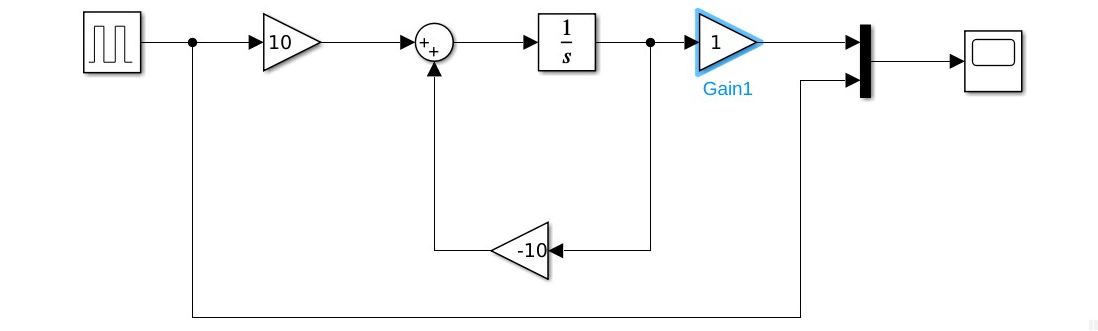
\includegraphics[width=1\linewidth]{"Code/Fig/part2_2_slx.png"} % Does not have to be a .pdf, can be another image file
				\caption{Simulink Diagram for Step Input Response}
				\label{fig:slx_step_input_diagram}
			\end{figure}	
			%%% Insert Figure Here as a image File %%%
			\begin{figure}[H]
				\centering
				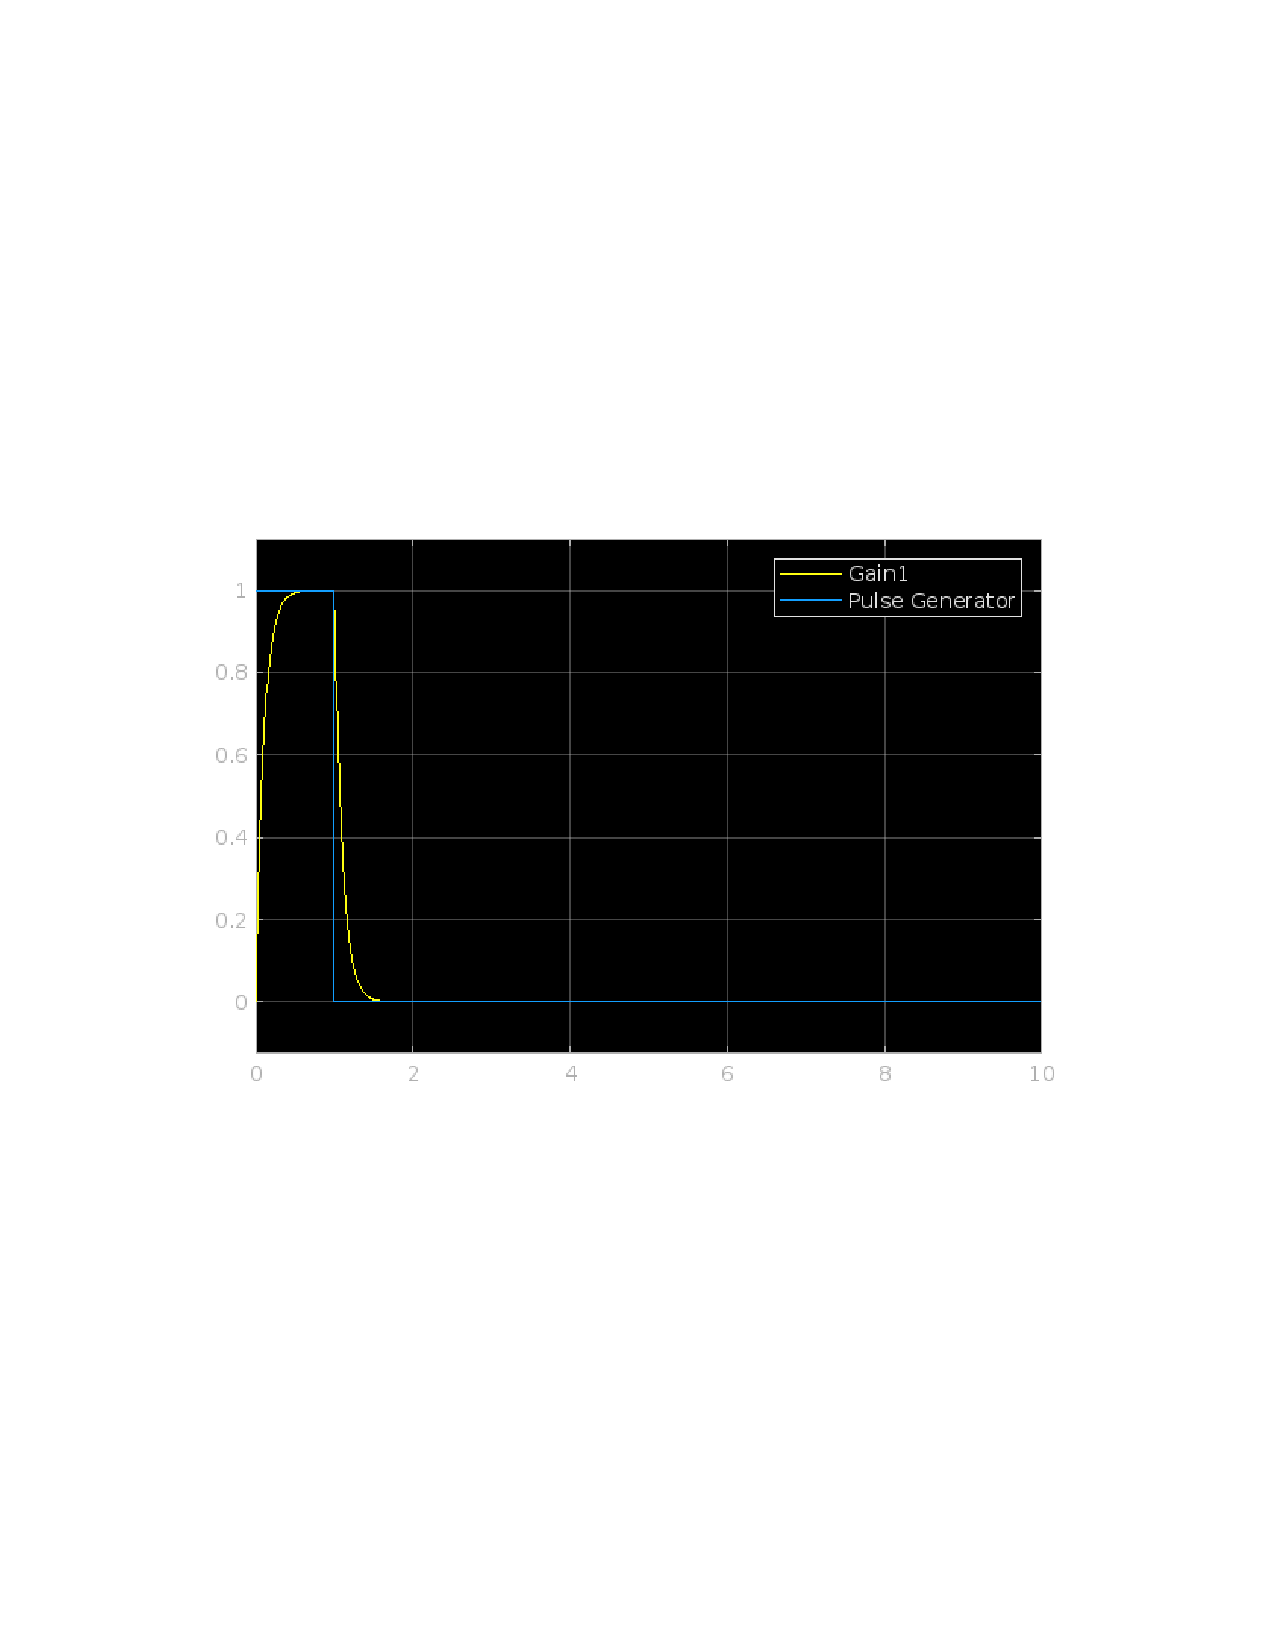
\includegraphics[width=0.8\linewidth]{"Code/Fig/step_input_output.png"} 
				\caption{Oscilloscope Output of Step Input Response}
				\label{fig:slx_step_input_output}
			\end{figure}
			% Answer questions pertaining to the section below
			After $t$ $\approx$ 0.6, the step input behaves as a zero input response. The curve settles at $\approx$ 1.2. Steady state is achieved in $\approx$ 0.6 seconds compared to $\tau$ being 0.15 seconds. Given that $T_{s}$ $\approx$ 4$\tau$, $T_{s}$ aligns with what was calculated.
			The gain of the response with an input of 1 has a magnitude of $\approx$ 1. This aligns with the value calculated in the pre-lab
		\subsection{Forced Response: Sinusoidal Input}
			\begin{figure}[H]
				\centering
				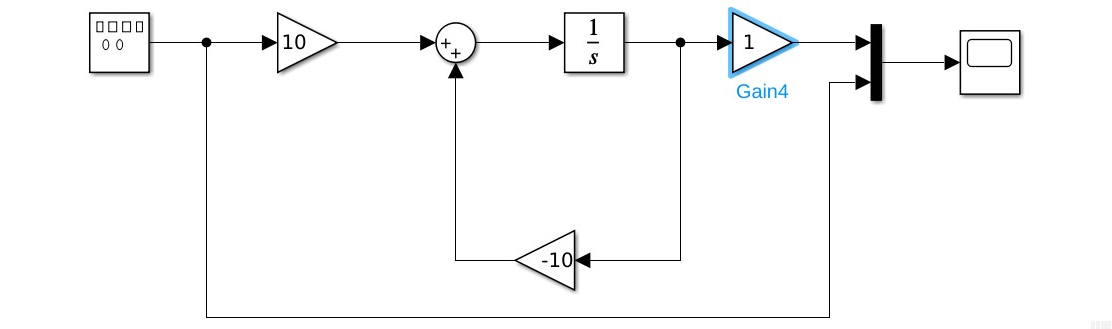
\includegraphics[width=1\linewidth]{"Code/Fig/part2_3_slx.png"} % Does not have to be a .pdf, can be another image file
				\caption{Simulink Diagram for Sinusoidal Input Response}
				\label{fig:slx_sine_input_diagram}
			\end{figure}
			%%% Insert Figure Here as a image File %%%		
%			\begin{figure}[H]
%				\centering
%				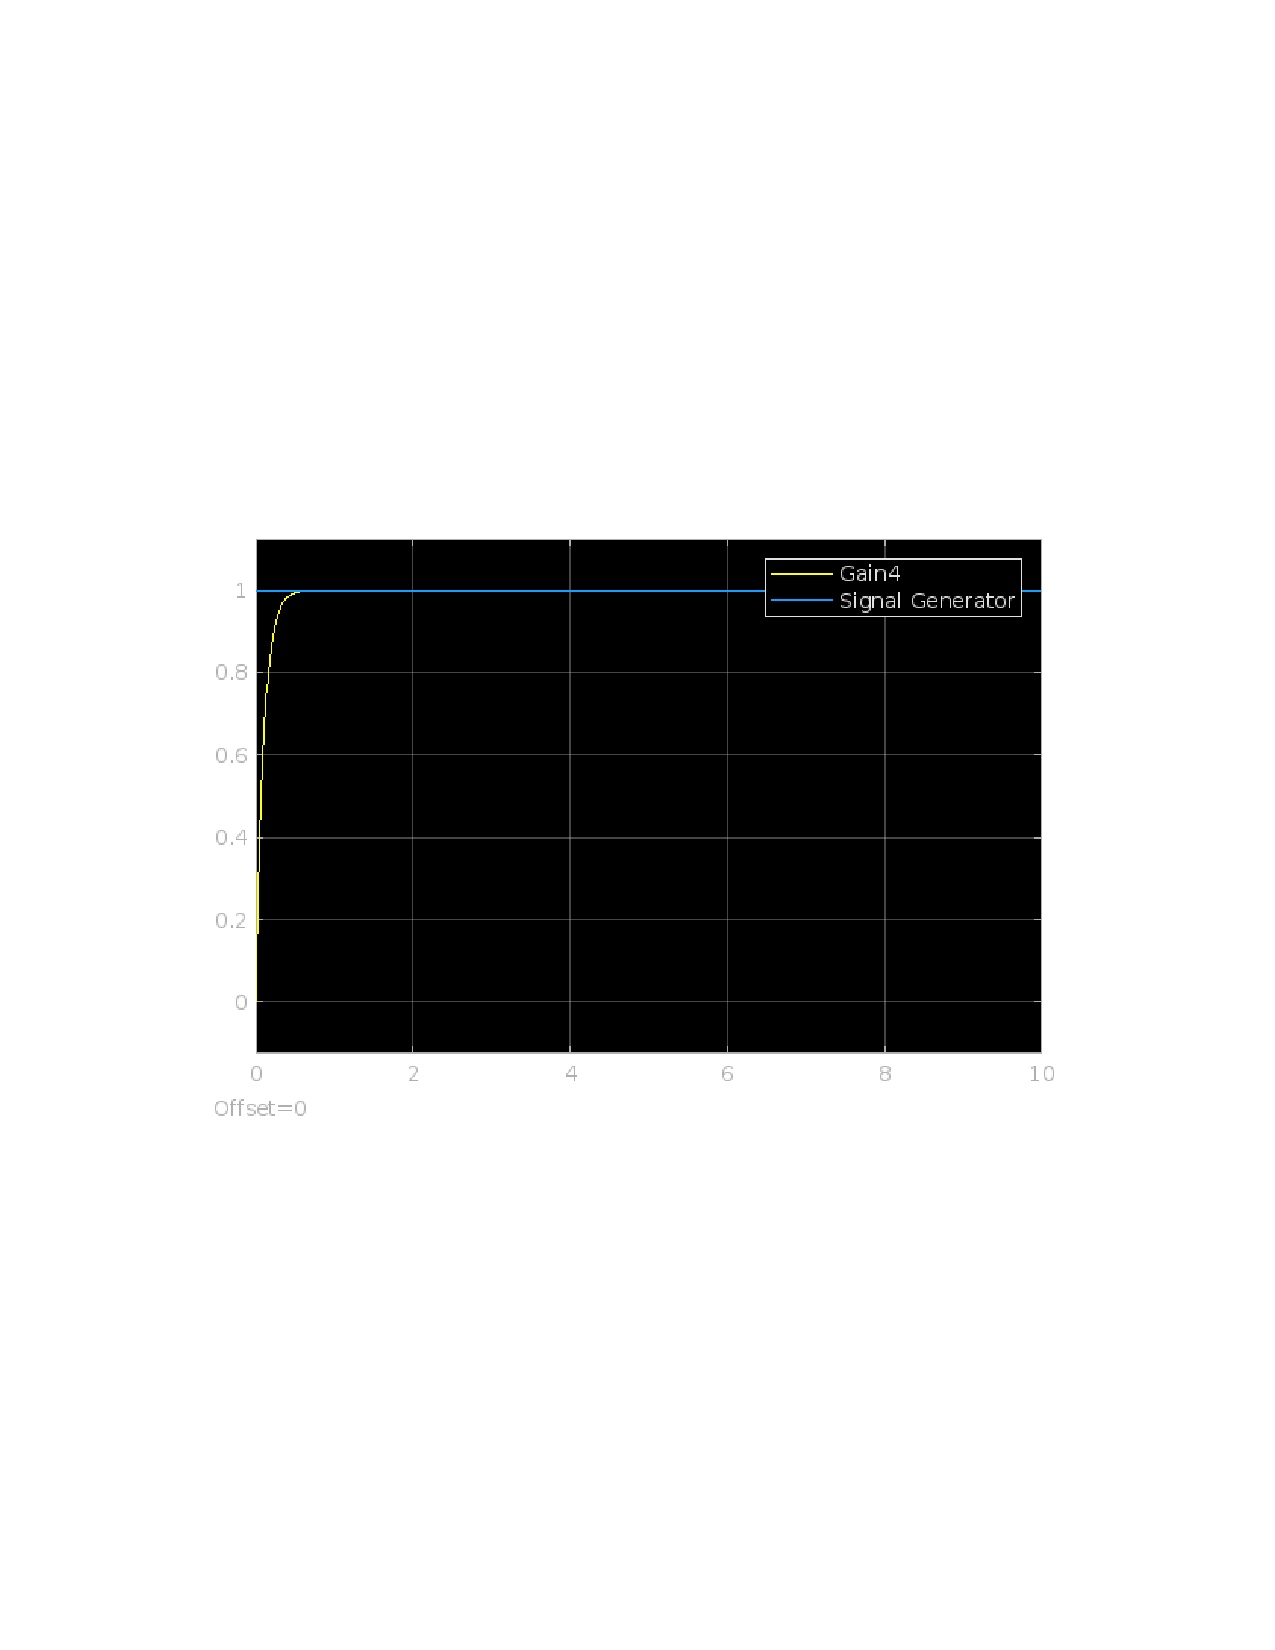
\includegraphics[width=1\linewidth]{"Code/Fig/sine_input_output_w_0.png"} 
%				\caption{Oscilloscope Output of Sinusoidal Input Response $\omega$ = 0.00}
%				\label{fig:slx_sine_input_output_w_0}
%			\end{figure}	
%			Magnitude and Phase are near identical.
			%%% Insert Figure Here as a image File %%%
			\begin{figure}[H]
				\centering
				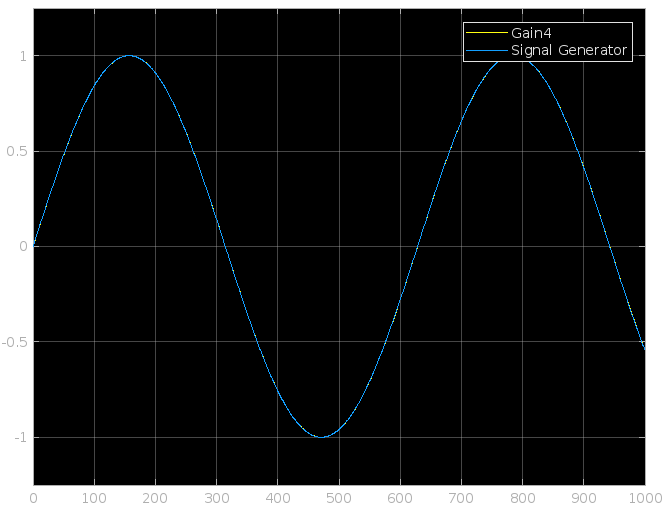
\includegraphics[width=1\linewidth]{"Code/Fig/sine_input_output_w_0_01.png"} 
				\caption{Oscilloscope Output of Sinusoidal Input Response $\omega$ = 0.01}
				\label{fig:slx_sine_input_output_w_0_01}
			\end{figure}
		
			\begin{figure}[H]
				\centering
				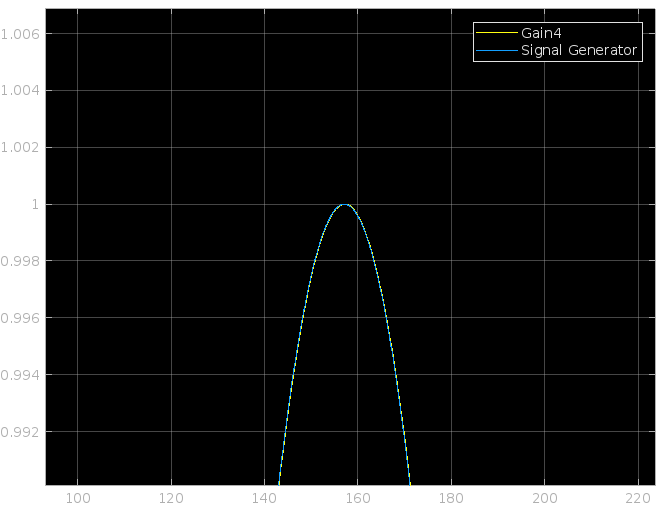
\includegraphics[width=1\linewidth]{"Code/Fig/sine_input_output_w_0_01_zoom.png"}
				\caption{Oscilloscope Output of Sinusoidal Input Response $\omega$ = 0.01 Overlap}
				\label{fig:sineinputoutputw001zoom}
			\end{figure}
				
			The sinusoidal input and output signals depicted in Figures \ref{fig:slx_sine_input_output_w_0_01} and \ref{fig:sineinputoutputw001zoom} exhibits identical magnitude and phase characteristics. This outcome aligns with the previously conducted frequency response analysis using a Bode plot. As evident in the figure, the blue and yellow lines, representing the input and output respectively, completely overlap, signifying perfect matching in both amplitude and phase characteristics.
			%%% Insert Figure Here as a image File %%%
			\begin{figure}[H]
				\centering
				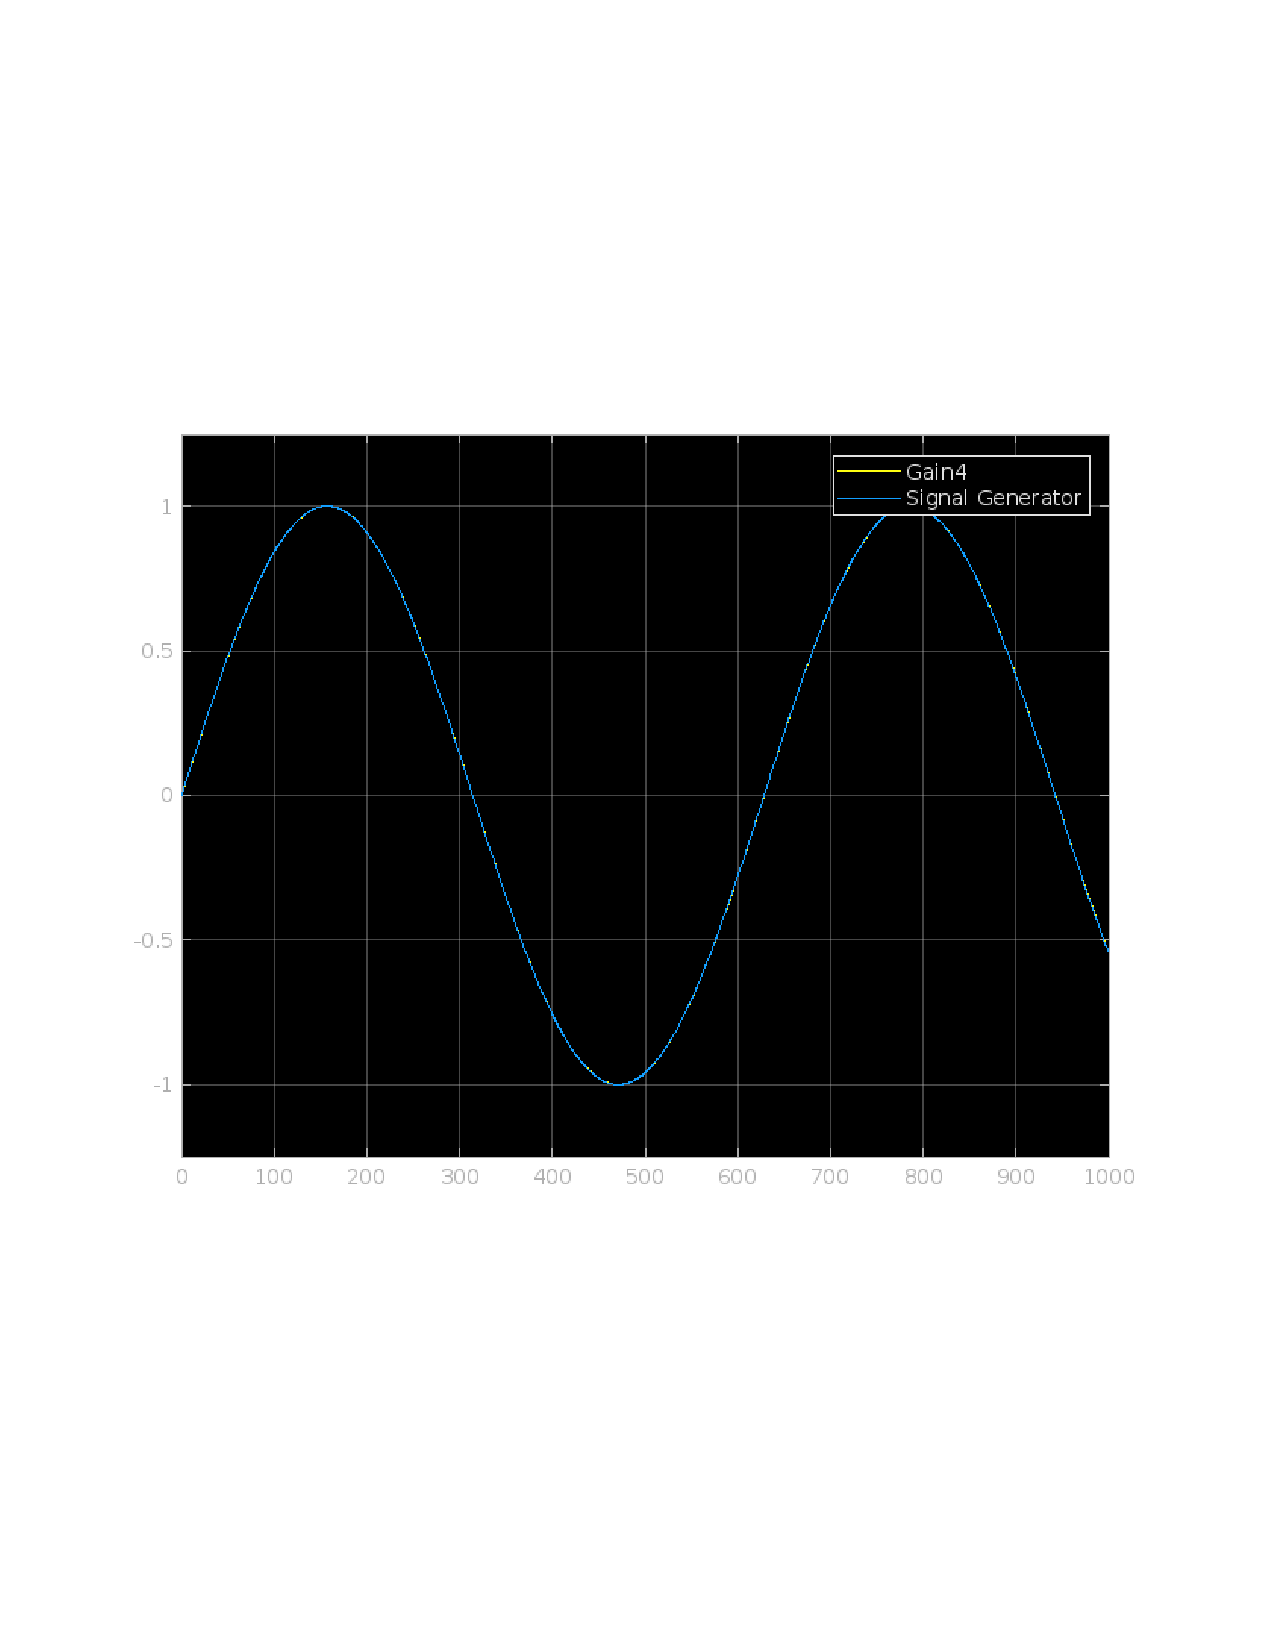
\includegraphics[width=1\linewidth]{"Code/Fig/sine_input_output_w_0_1.png"} 
				\caption{Oscilloscope Output of Sinusoidal Input Response $\omega$ = 0.10}
				\label{fig:slx_sine_input_output_w_0_10}
			\end{figure}	
			The sinusoidal input and output signals depicted in Figure \ref{fig:slx_sine_input_output_w_0_10} and exhibits identical magnitude and phase characteristics. This outcome aligns with the previously conducted frequency response analysis using a Bode plot. As evident in the figure, the blue and yellow lines, representing the input and output respectively, completely overlap, signifying perfect matching in both amplitude and phase characteristics.
			%%% Insert Figure Here as a image File %%%
			\begin{figure}[H]
				\centering
				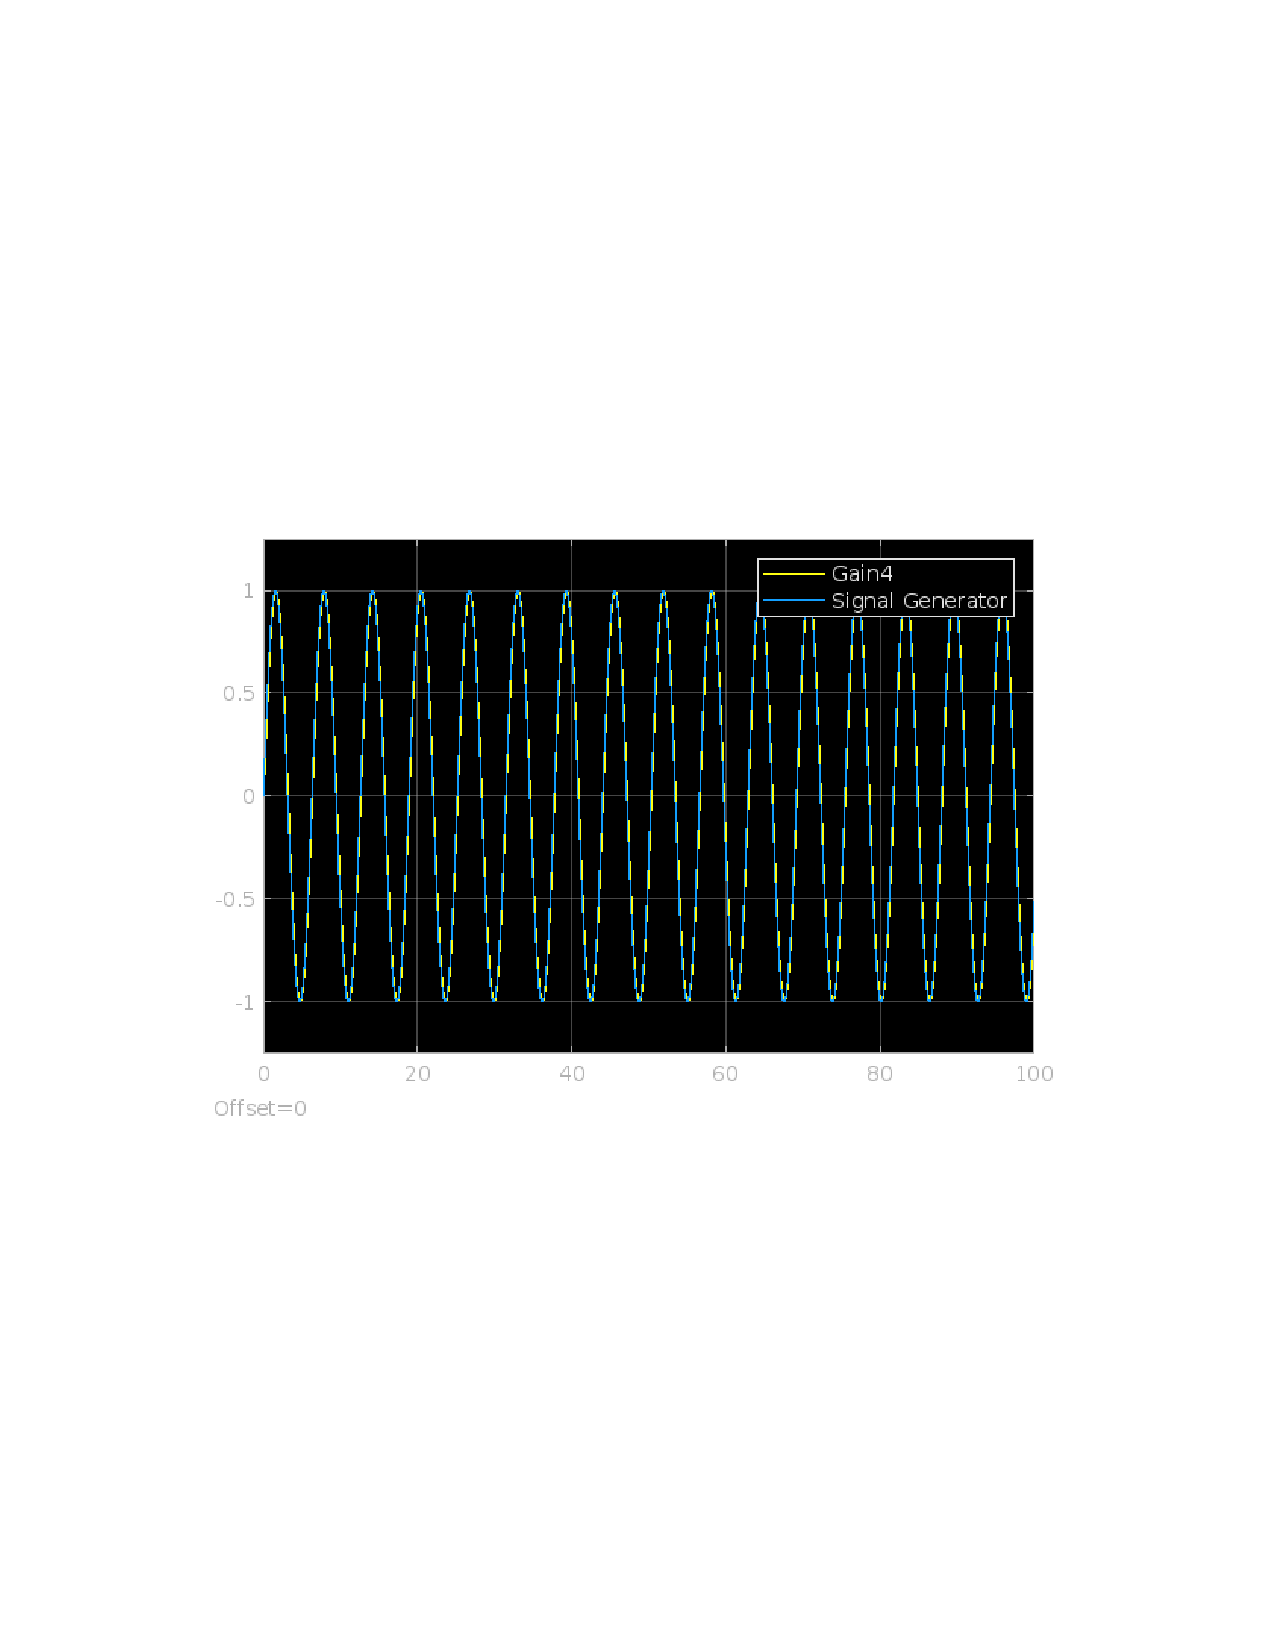
\includegraphics[width=1\linewidth]{"Code/Fig/sine_input_output_w_1.png"} 
				\caption{Oscilloscope Output of Sinusoidal Input Response $\omega$ = 1.00}
				\label{fig:slx_sine_input_output_w_1}
			\end{figure}
			The sinusoidal input and output signals depicted in Figure \ref{fig:slx_sine_input_output_w_0_1} and exhibits identical magnitude and phase characteristics. This outcome aligns with the previously conducted frequency response analysis using a Bode plot. As evident in the figure, the blue and yellow lines, representing the input and output respectively, completely overlap, signifying perfect matching in both amplitude and phase characteristics.
			%%% Insert Figure Here as a image File %%%
			\begin{figure}[H]
				\centering
				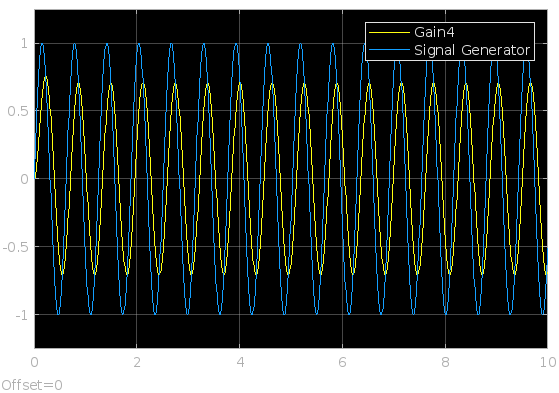
\includegraphics[width=1\linewidth]{"Code/Fig/sine_input_output_w_10.png"} 
				\caption{Oscilloscope Output of Sinusoidal Input Response $\omega$ = 10.00}
				\label{fig:slx_sine_input_output_w_10}
			\end{figure}
			\begin{figure}[H]
				\centering
				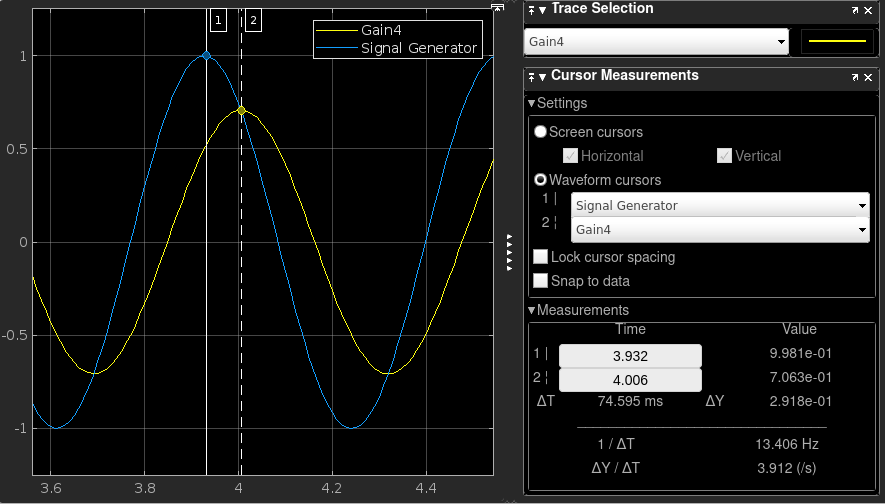
\includegraphics[width=1\linewidth]{"Code/Fig/w_10_mag.png"} 
				\caption{Oscilloscope Gain of Sinusoidal Input Response $\omega$ = 10.00}
				\label{fig:slx_sine_input_output_w_10_mag}
			\end{figure}
			\begin{figure}[H]
				\centering
				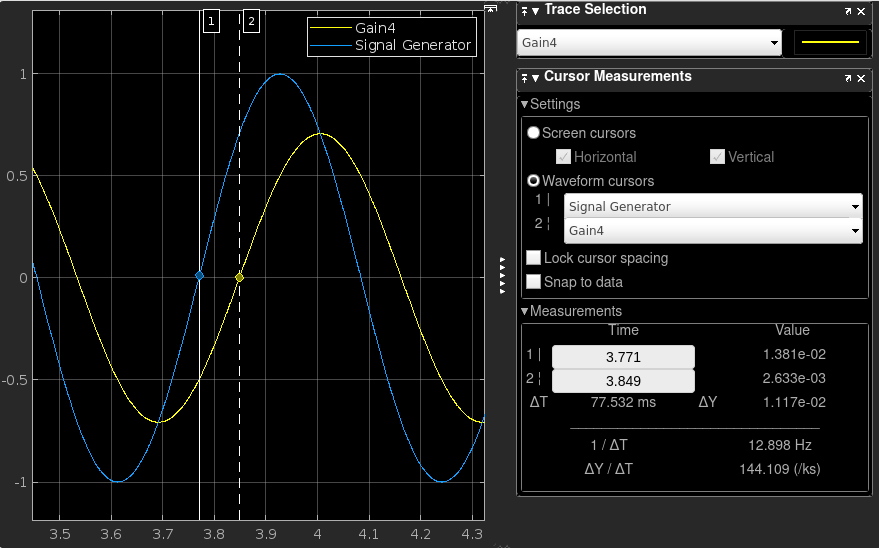
\includegraphics[width=1\linewidth]{"Code/Fig/w_10_ang.png"} 
				\caption{Oscilloscope Phase Shift of Sinusoidal Input Response $\omega$ = 10.00}
				\label{fig:slx_sine_input_output_w_10_ang}
			\end{figure}		
			The magnitude difference $\frac{0.708}{0.998}$ is $\approx$ .0708 and the phase shift is = $\omega \times \Delta T$ = 10 $\times$ -0.0775 s  $\approx$ -0.775 rad.
			%%% Insert Figure Here as a image File %%%
			\begin{figure}[H]
				\centering
				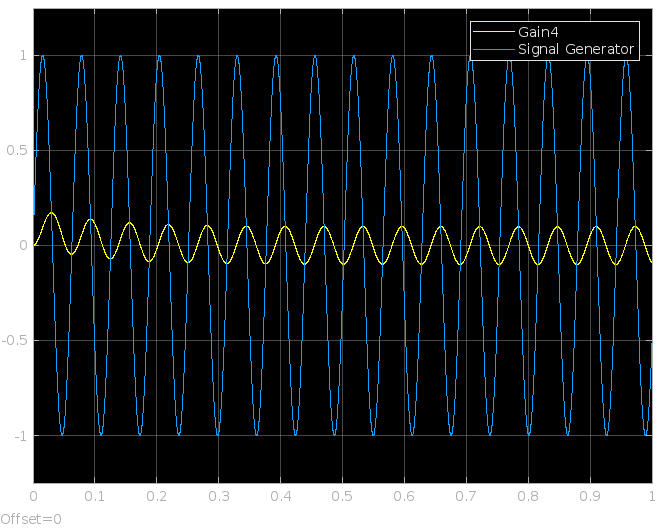
\includegraphics[width=1\linewidth]{"Code/Fig/sine_input_output_w_100.png"} 
				\caption{Oscilloscope Output of Sinusoidal Input Response $\omega$ = 100.00}
				\label{fig:slx_sine_input_output_w_100}
			\end{figure}
			\begin{figure}[H]
				\centering
				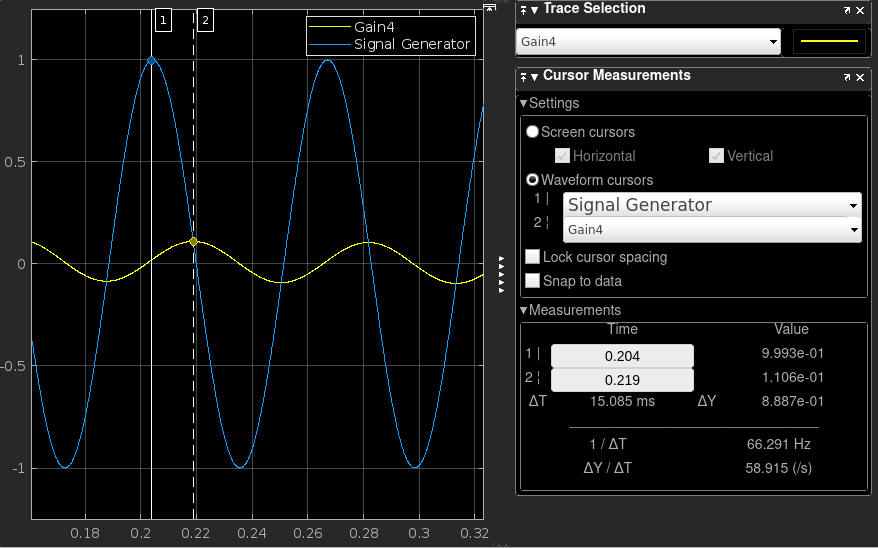
\includegraphics[width=1\linewidth]{"Code/Fig/w_100_mag.png"} 
				\caption{Oscilloscope Gain of Sinusoidal Input Response $\omega$ = 100.00}
				\label{fig:slx_sine_input_output_w_100_mag}
			\end{figure}
			\begin{figure}[H]
				\centering
				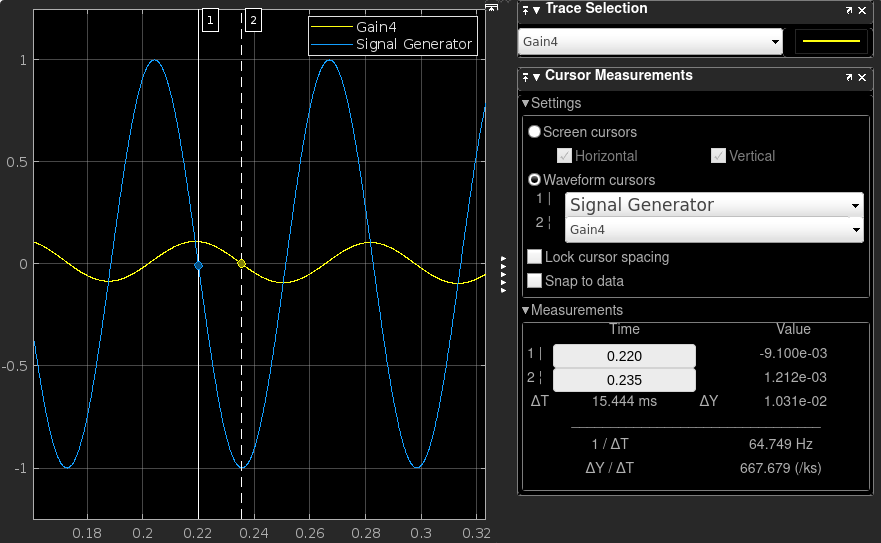
\includegraphics[width=1\linewidth]{"Code/Fig/w_100_ang.png"} 
				\caption{Oscilloscope Phase Shift of Sinusoidal Input Response $\omega$ = 100.00}
				\label{fig:slx_sine_input_output_w_100_ang}
			\end{figure}		
			The magnitude difference $\frac{0.111}{0.999}$ is $\approx$ 0.11 and the phase shift is = $\omega \times \Delta T$ = 100 $\times$ -0.0154 s  $\approx$  -1.54 rad. \\
			% Answer questions pertaining to the section below
			The frequency and phase are similar to those predicted in Table \ref{tab:rc} and Figure \ref{fig:bode}.  
		
	\section{Conclusion}
	%%% PUT CONCLUSION HERE %%
	The comprehensive exploration and modeling of a first-order RC circuit in this laboratory exercise, employing MATLAB and Simulink for simulation, yielded insightful results. The simulation outcomes effectively corroborate the anticipated frequency response and Bode plots analysis. At nominal frequencies, the circuit demonstrated conventional decay characteristics. However, as frequencies escalated, the capacitor's influence became more pronounced, altering both magnitude and phase of input signals. Notably, the circuit exhibited low-pass behavior with negligible distortion for frequencies below $\omega$ $\leq$ 1, effectively attenuating signals beyond $\omega$ $\geq$ 100. This validation underscores the circuit's intended functionality and its applicability within specified frequency ranges.

\end{document}